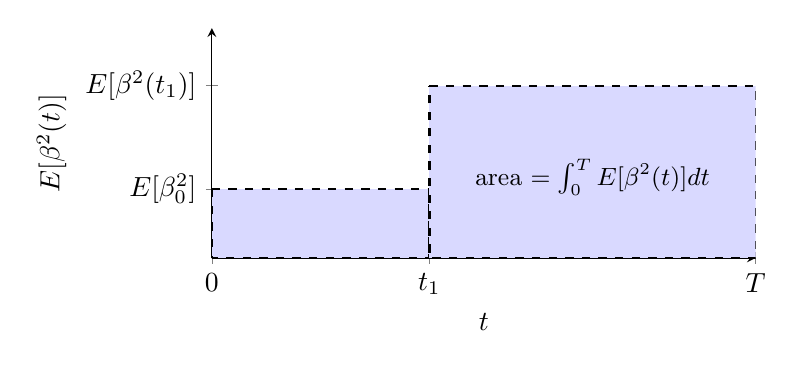
\begin{tikzpicture}
\begin{axis}[width=0.7\textwidth,height=4.5cm,xlabel={$t$},ylabel={$\mathbb{E}[\beta^2(t)]$},xmin=0,xmax=1,ymin=0,ymax=2,xtick={0,0.4,1},xticklabels={$0$,$t_1$,$T$},ytick={0.6,1.5},yticklabels={$\mathbb{E}[\beta_0^2]$,$\mathbb{E}[\beta^2(t_1)]$},axis lines=left]
\addplot[black,dashed,thick,fill=blue!15] coordinates {(0,0.6)(0.4,0.6)} \closedcycle;
\addplot[black,dashed,thick,fill=blue!15] coordinates {(0.4,1.5)(1,1.5)} \closedcycle;
\node at (axis cs:0.7,0.7) {\small area $=\int_0^T\mathbb{E}[\beta^2(t)]dt$};
\end{axis}
\end{tikzpicture}
